\section{РЕАЛИЗАЦИЯ}

\subsection{Используемые технологии}

Таким образов в программу вошли классические алгоритмы численных методов, такие как методы матричной алгебры, методы
Ньютона и так далее. Для её написания были использованы \textit{язык программирования C++}, \textit{фреймворк QT}
и автоматизатор сборок проектов \textit{CMake}. Полный список технологий и алгоритмов предоставлен на рисунке \ref{fig:stack}.
Для поиска ошибок и утечек памяти применилась связка из отладчика \textit{GDB} и профилировщика \textit{Valgrind}. 

\begin{figure}
    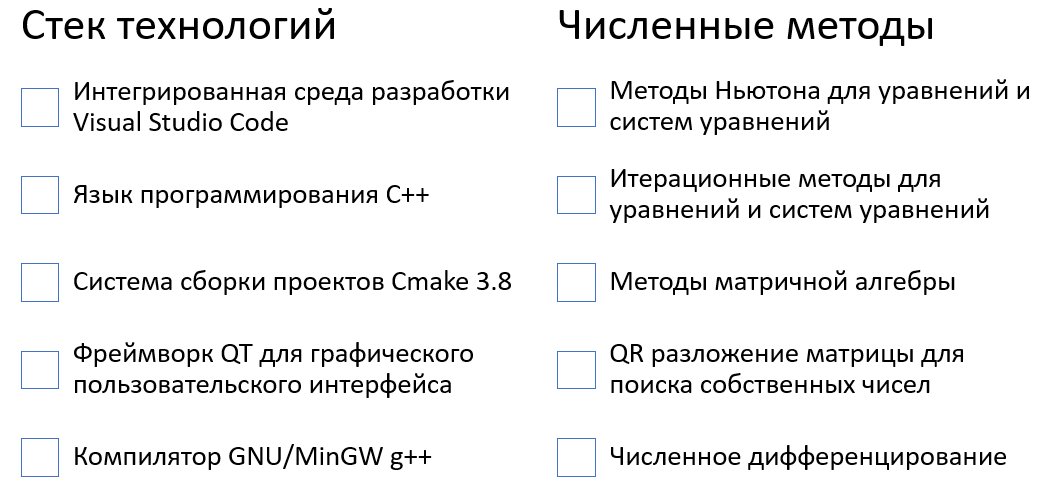
\includegraphics[width=15cm]{2-04-realisation}
    \caption{Технологии и алгоритмы}
    \label{fig:stack}
\end{figure}

Фреймворк QT нужен для разработки кроссплатформенного программного обеспечения с графическим интерфейсом \cite{Wikipedia5}. Собственная
среда \textit{QT Designer} позволяет строить пользовательский графический интерфейс при помощи множества инстументов.

Программа для автоматизации сборок проектов CMake самой сборкой не занимается, а лишь генерирует файлы сборки из предварительно
написанного файла сценария \textit{CMakeLists.txt} и предоставляет простой единый интерфейс управления \cite{Wikipedia4}. Возможность
нескольких вариаций сборок с разными ключами компиляции, автоматизация процесса установки пакетов и кроссплатформенность делают CMake
отличным выбором для разработки.

Отладчик GDB позволяет отслеживать различные ошибки при работе программы. GDB предлагает обширные средства для слежения и
контроля за выполнением исполняемых файлов \cite{Wikipedia2}. При создании больших проектов может возникнуть множество неочевидных
ошибок, которые приходится отлавливать благодаря специальным программам, к числу которых и относится GDB.

Если GDB нужен для поиска ошибок, связанных с переменными, то профилировщик Valgrind нужен для поиска ошибок связанных с памятью.
К числу таких ошибок относятся: утечки памяти, ошибка сегментации, попытки использования неинициализированной памяти и так далее.
Вся эта работа выполняется при помощи инструмента \textit{Memcheck}. Так же Valgrind может предоставить инструменты для профилировки,
такие как \textit{Cachegrind}, \textit{Callgrind} и так далее \cite{Wikipedia3}.

После рассмотрения используемых технологий можно перейти к алгоритму выполнения программы.
Общий алгоритм работы, показан на рисунке \ref{fig:sheme}.

\begin{figure}
    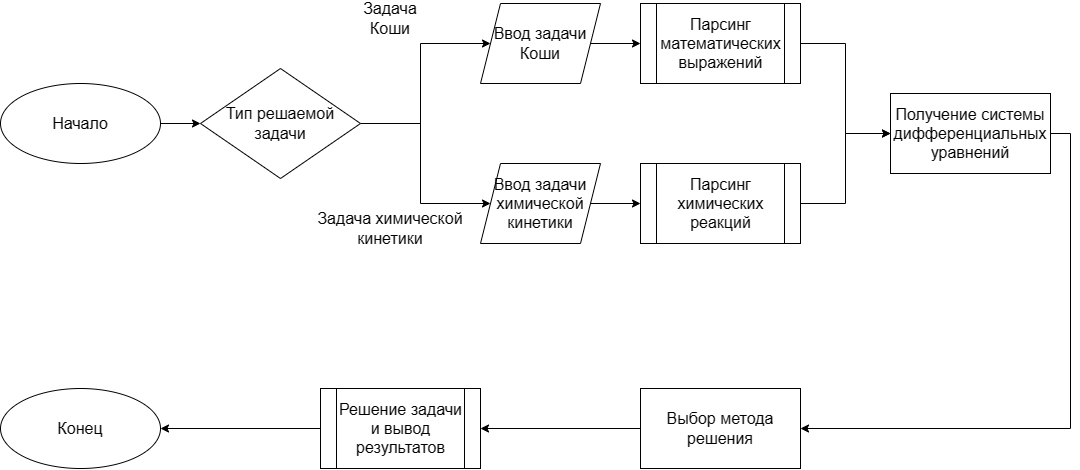
\includegraphics[width=15cm]{2-04-scheme}
    \caption{Алгоритм работы программы}
    \label{fig:sheme}
\end{figure}

Сначала выбирается тип решаемой задача, после чего всплывает форма с соответствующими текстовыми полями для ввода. После этого, в
зависимости от типа решаемой задачи, происходит обработка ввода и формирование СДУ, которые решаются
выбранным методом. Результаты работы выводятся либо на экран, либо в отдельном файле.

Для решения ОДУ был реализован большой перечень как явных так и неявных методов с различным порядком точности. Для удобства разработки
и тестирования, программа была поделена на множество отдельных модулей. Далее приведено детальное рассмотрение каждого из них.

\subsection{Общие алгоритмы и структуры}

В данном подразделе перечислены основные алгоритмы и структуры, которые использовались в остальных модулях. Сюда вошли алгоритмы
LU-разложения матрицы, QR алгоритм нахождения собственных чисел матрицы, алгоритмы дифференцирования с разным порядком точности. Для
работы с таблицами Бутчера и алгоритмами решения СНУ был реализован собственный класс матрицы с базовой матричной алгеброй.

\textit{Матрица}

Реализация матрицы в данной работе представляет из себя класс, содержащий одномерный массив $n \times m$, где $n, m$ ~--- размеры
матрицы. В комплект к ней входят простейшие оперции матричной алгебры, такие как умножение, сложение, возведение в степень и так далее.
В дополнение к этим операциям были реализованы алгоритм нахождения обратной матрицы и определителя при помощи LU-разложения.

Матрица используется для хранения таблиц Бутчера, вычисления Якобиана, построения матрицы системы уравнений и дальнейшее вычисление
числа жёсткости и так далее. Дополнительно были реализованы возможность проверки матрицы на симметричность, квадратность и
операции добавления/удаления строк/столбцов.

\textit{LU алгоритм}

LU-разложение матрицы A представляет собой разложение матрицы A в
произведение нижней и верхней треугольных матриц, т.е. $A = LU$, где $L$ ~--- нижняя треугольная матрица на диагонали которой
стоят единицы, $U$ ~--- верхняя
треугольная матрица. LU–разложение может быть использовано при решении
систем линейных алгебраических уравнений вида $Ax = b$. Полученное LU-разложение может быть так же использовано для вычисления определителя
матрицы по формуле.
\begin{equation}
    det(A) = det(L)det(U) = (\prod\limits_{i = 1}^nL_{ii})(\prod\limits_{i = 1}^nU_{ii}) = \prod\limits_{i = 1}^nU_{ii},
    \label{eq:Det}
\end{equation}

где $n$ ~--- размер квадратной матрицы.

Для нахожения обратной матрицы из задачи $AX = E$, где $A$ ~--- исходная матрица, $X$ ~--- обратная матрица, $E$ ~--- единичная
матрица, составляется $n$ систем уравнений:
\begin{equation}
    \begin{gathered}
        AX_i = e_i,  i = 1, ..., n,
    \end{gathered}
    \label{eq:Reverse}
\end{equation}

где $X_i$ ~--- вектор-столбец обратной матрицы с индексом $i$, $e_i$ ~--- вектор-столбец единичной матрицы с индексом $i$.

Нахождение обратной матрицы сводится к решению $n$ уравнений с одной матрицей и разными правыми частями.

\textit{QR алгоритм}

При решении полной проблемы собственных значений для несимметричных
матриц эффективным является подход, основанный на приведении матриц к подобным, 
имеющим треугольный или квазитреугольный вид. Одним из наиболее распространенных
методов этого класса является QR-алгоритм.

В основе QR-алгоритма лежит представление матрицы в виде

\begin{equation}
A = QR,
\label{eq:QRCommon1}
\end{equation}

где - $Q$, ортогональная матрица ($Q^{-1} = Q^T$), а
$R$ ~--- верхняя треугольная. Такое разложение
существует для любой квадратной матрицы. Одним из возможных подходов к построению
QR разложения является использование преобразования Хаусхолдера. Преобразование Хаусхолдера осуществляется с использованием 
матрицы
Хаусхолдера, имеющей следующий вид:
\begin{equation}
    H = E - \dfrac{2}{\nu^T\nu}\nu\nu^T,
    \label{eq:QRCommon2}
\end{equation}

где $E$ ~--- единичная матрица, $\nu$ ~--- произвольный ненулевой вектор-столбец.
Само преобрахование имеет вид

\begin{equation}
    A_{i + 1} = H_iA_i
    \label{eq:QRAlgo}
\end{equation}

Матрица $Q$ является произведением матриц Хаусхолдера, полученных на каждом шаге. Матрица $R$, как $A_{n-1}$.

\begin{equation}
    \begin{gathered}
        Q = H_1H_2...H_{n-1}, R = A_{n - 1}
    \end{gathered}
    \label{eq:QFind}
\end{equation}

Код реализации алгоритма продемонстрирован на рисунке \ref{src:QR}.

\begin{figure}
    \lstinputlisting[language=C++]{inc/Code/QR.cpp}
    \caption{Код QR алгоритма}
    \label{src:QR}
\end{figure}

\textit{Дифференцирование}

Для численного дифференцирования был разработана функция, получающая  получающая в качестве аргументов функция для дифференцирования,
точку, в которой необходимо продифференцировать функцию и схему дифференцирования. Как можно заметить из формул (\ref{eq:Diff}), все
эти схемы являются достаточно похожими, поэтому появилась идея представления этих схем в следующем виде:

\begin{equation}
    y' = \frac{a_1y_{i-n+1} + a_2y_{i-n+2} + ... + a_{2n-1}y_{i+n-1}}{ch^p}
    \label{eq:DiffCommon}
\end{equation}

где $n$ ~--- количество точек аппроксимации.

При таком представлении все схемы можно реализовать при помощи одномерного массива коэффициентов.

$$
[a_1, a_2, ..., a_{2n - 1}, c, p]
$$

где $a_i$ ~--- коэффициенты для точек, $c$ ~--- коэффициент перед шагом в знаменателе, $p$ ~--- степень шага. Такой подход позволяет
быстро дополнять текущий набор схем новыми. Помимо этого избегается дублирование одинакого кода.
Так, например, вторая 4-х точечная схема 

\begin{equation}
    y_i' = \frac{-11y_{i} + 18y_{i+1} - 9y_{i+2} + 2y_{i+3}}{6h}
    \label{eq:Diff1-4}
\end{equation}

может быть представлена в следующем виде:

$$
[0, 0, 0, -11, 18, -9, 2, 6, 1]
$$

\textit{Вычисление жёсткости}

Для вычисления числа жёсткости по формуле (\ref{eq:tough}) нужно построить матрицу Якоби для системы и найти её собственные числа.

Коэффициентом жёсткости задачи называется отношение максимального модуля действительной части собственных чисел матрицы Якоби к
минимальной при условии, что все действительные части собственных чисел меньше нуля. Собственные числа данной матрицы находятся
при помощи алгоритма QR-разложения. Для построения данной матрицы используется схема дифференцирования по 4-м точкам.

%разбить на 3 этапа
\subsection{Графический пользовательский интерфейс}

Для ввода задачи была реализована специальная форма с использованием фреймворка QT. Её внешний вид представлен на рисунке \ref{fig:forma1}.
Преобразование строк в функции происходит при помощи парсера математических выражений.

\begin{figure}
    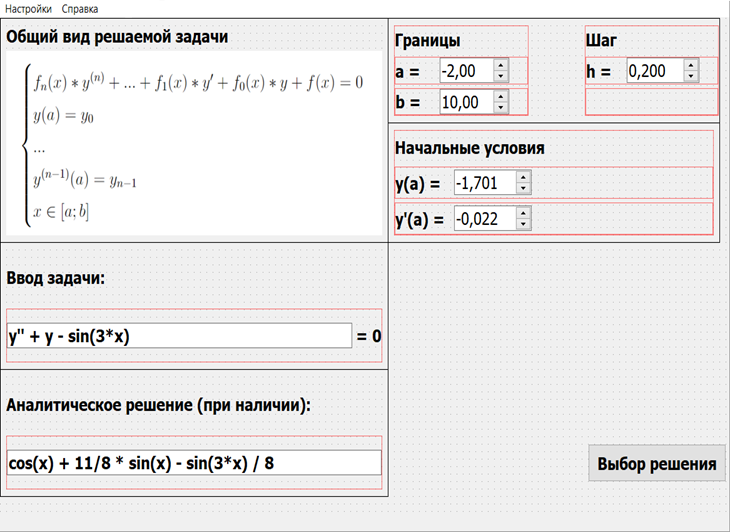
\includegraphics[width=15cm]{2-04-forma}
    \caption{Вид интерфейса для ввода задачи Коши}
    \label{fig:forma1}
\end{figure}

После ввода задачи, аналитического решения (при наличии), начальных условий и границ интегрирования требуется выбрать метод решения.
Перед выбором решения идёт анализ задачи на жёсткость и если число жёсткости задачи велико ($> 100$), то выбор методов ограничивается
явными высоких порядков, неявными и вложенными, иначе выбор методов не ограничивается.

% \begin{figure}
%     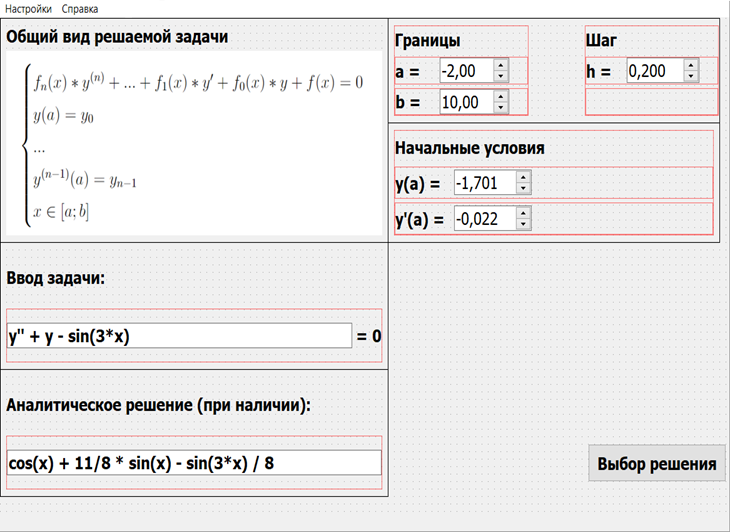
\includegraphics[width=15cm]{2-04-forma}
%     \caption{Вид интерфейса для ввода задачи Коши}
%     \label{fig:forma2}
% \end{figure}

Результаты вичислений либо сохраняются в отдельном файле, либо выводятся на экран.

\subsection{Парсер математических выражений}

При режиме работы с задачей Коши от пользователя требуется ввести задачу и аналитическое решение (при наличии). 

Для обработки строк с задачей был реализован парсер математических выражений. Принцип его работы следующий: проводится лексический
анализ строки, описывающей функцию, и строится дерево
математических выражений, содержащее функции и операторы математических выражений в качестве узлов
и числовые константы с переменными в качестве листьев.

Реализация в виде дерева была выбрана по нескольким причинам:

\begin{itemize}
    \item лёгкость в написании,
    \item простота в расширении функционала,
    \item некоторые операции (поиск коеффициентов при переменной, выделение поддерева и т.д.) легче выполнять при работе с деревом.
\end{itemize}

Интерфейс парсера позволяет использовать его как функтор, принимающий либо одну переменную, либо массив переменных. Реализована поддержка
базовых функций и числовых констант. Так же есть возможность добавления пользовательских параметров и констант.

Для сравнения эффективности реализации было проведено тестирование на модельных функциях с использованием парсера и обычных
статических функций. Сравнения по времени приведены в таблице \ref{tab:Banchmark}.

\begin{table}    
    \caption{Таблица сравнения статических функций и парсера}
    \begin{tabularx}{\textwidth}{|X|c|c|}
    \hline
    Уравнение & Статическая функция (ms) & Парсер (ms)\\
    \hline
    $x + 2$ & 18 & 35\\
    \hline
    $\sin(\cos(x)) + \cos(\cos(x))$ & 253 & 492\\
    \hline
    $\sin(-x) + \ln(e^{10}) + \arccos((-1)^x)$ & 623 & 1007\\
    \hline
    $\dfrac{11 - x^3 (3x - 8)}{12(x - 2)^2 (x - 3)}$ & 23 & 172\\
    \hline
    $x\exp(\dfrac{1}{x})$ & 29 & 109\\
    \hline
    $\exp(x\sin(\ln(x)) + x)$ & 393 & 385\\
    \hline
    $\dfrac{x^3}{4} - \dfrac{1}{x}$ & 22 & 108\\
    \hline
    $1 + \ln(abs(x))$ & 40 & 65\\
    \hline
    $\cos(\sqrt{4x}) + \sin(\sqrt{4x})$ & 303 & 349\\
    \hline
    $abs(x)^\frac{3}{2}$ & 249 & 293\\
    \hline
    \end{tabularx}
    \label{tab:Banchmark}
\end{table}

На данной таблице видно, что парсер уступает по скорости обычным функциям в 1.5-2 раза. Это связано с тем, что при работе с деревом
приходится проходить по указателям к нижним узлам, что сильно замедляет работу алгоритма.
Так же была протестирована реализация парсинга математических выражений при помощи обратной польской записи, однако она давала небольшой
выигрыш по времени при урезанном функционале.

Рисунок \ref{src:FuncMaker} показывает листинг с примерами использования парсера.

\begin{figure}
    \lstinputlisting[language=C++]{inc/Code/FuncMaker.cpp}
    \caption{Пример использования парсера}
    \label{src:FuncMaker}
\end{figure}

В дальнейшем планируется добавление возможность аналитического дифференцирования функций, добавление пользовательских функций от 2-х и
более перменных и дальнейшая оптимизация скорости работы парсера.

\subsection{Парсер химичесских уравнений}

Химические уравнения обычно записываются в виде

\begin{equation}
    Sub_1 + Sub_2 \Longleftrightarrow Sub_3 + Sub4,
    \label{eq:Chemic}
\end{equation}

где $Sub_i$ ~--- некоторые вещества. Помимо формул, для моделирования реакций нужно знать термодинамические свойства веществ \cite{book3}
и Аррениусовские константы скоростей для каждой реакции \cite{book8}.

На основе этих данных формируется СДУ, порядок которой равен числу веществ, участвующих в реакциях. Подробнее про это расписано в
следующих разделах.

\subsection{Реализация методов решения}

Как уже говорилось выше, все методы семейства Рунге-Кутты можно представить в виде таблиц Бутчера. В связи с этим появилась идея
реализовать алгоритм, принимающий в качестве аргументов задачу и таблицу Бутчера и возвращающий решение в виде таблицы с координатами.
Благодаря этому алгоритму добавлять
новые методы не вызывает никаких сложностей. Используемые методы перечислены на рисунке \ref{fig:SolveMethods}.
Всего в данной работе используется 62 схемы со 2 по 6 порядок точности.

\begin{figure}
    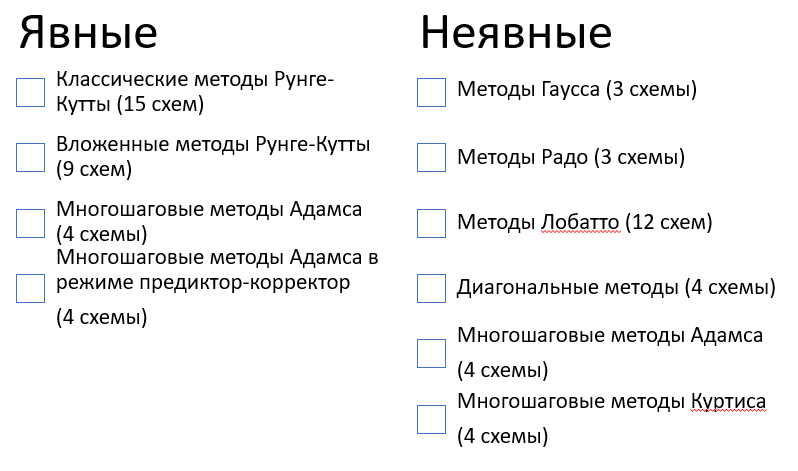
\includegraphics[width=15cm]{2-04-methods}
    \caption{Методы решения}
    \label{fig:SolveMethods}
\end{figure}

По желанию пользователя можно добавить другой метод при помощи специального конструктора.

\subsection{Генерация отчёта}

При генерации отчёта учитывается количество уравнений, тип решаемой задачи, количество шагов интегрирования. При решении задач химической
кинетики аналитическое решение не вводится. Отдельно выводятся графики изменения плотности и температуры. В обоих типах задач при
большом количестве точек их число уменьшается в несколько раз (оставляется каждая вторая или каждая третья). На рисунке \ref{fig:report}
показан пример одной страницы отчёта.

\begin{figure}
    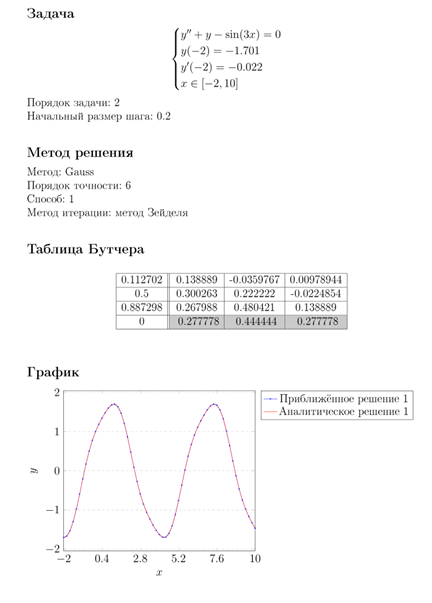
\includegraphics[width=10cm]{2-04-report}
    \caption{Пример страницы отчёта}
    \label{fig:report}
\end{figure}

Для версии программы без интерфейса отчёт выводится либо в текстовом виде, либо в TeX-файле.
